%% ------------------------------------------------------------------------- %%
\chapter{Planejamento e Execução do Estudo} 
\label{cap:qualitativo-planejamento}

Conduzir um estudo experimental em engenharia de software sempre foi uma
atividade difícil. Uma das razões para isso é o fator humano, muito presente 
no processo de desenvolvimento de software, como sugerido por métodos ágeis  em
geral \cite{AgileManifesto}. Dessa maneira, o paradigma de pesquisa analítico 
não é suficiente para investigar casos reais complexos envolvendo pessoas e 
suas interações com a tecnologia \cite{guidelines-case-study}.

Conforme apontado por Seaman \cite{seaman}, esses problemas já foram levantados
por muitos pesquisadores e, finalmente, tem-se considerado a influência de
problemas não-técnicos e a intersecção entre eles e a parte técnica
dentro da engenharia de software. 
Apesar disso, o número de estudos empíricos é ainda muito pequeno dentro da área
de pesquisa em ciência da computação: Sjoberg \textit{et al.} \cite{sjoberg} encontraram
apenas 103 experimentos em 5.453 artigos, e Ramesh \textit{et al.} \cite{ramesh}
identificaram menos de 2\% de experimentos envolvendo humanos e apenas 0.16\% 
estudos em campo dentre 628 artigos.

Uma pesquisa qualitativa é um meio para se explorar e entender a influência que 
indivíduos ou grupos atribuem a um problema social ou humano. O processo de
pesquisa envolve questões emergentes e procedimentos, dados geralmente colhidos
sob o ponto de vista do participante, com a análise feita de maneira indutiva
indo geralmente de um tema específico para um tema geral e com o pesquisador
fazendo interpretações do significado desses dados. Dados capturados por estudos
qualitativos são representados por palavras e figuras, e não por números.
O relatório final tem uma estrutura flexível e os pesquisadores que se
dedicam a esta forma de pesquisa apoiam uma maneira de olhar para a pesquisa que
honra o estilo indutivo, o foco em termos individuais, e a importância de mostrar a 
complexidade de uma situação \cite{creswell}. 

Conforme discutido no Capítulo \ref{cap:trabalhos-relacionados}, muitos 
trabalhos avaliaram TDD, e alguns deles relatam inclusive uma melhora
no projeto de classes, como um menor acoplamento, uma maior coesão, e até mesmo
mais simplicidade. 
Grande parte deles focam nos efeitos da prática no código final, mas poucos 
estudos tentam entender a possível influência da experiência
nos resultados encontrados, e como TDD e a prática de escrever o teste 
antes do código real realmente guiam o programador 
em direção a essas melhorias.

Para entendê-las, este estudo faz uso de uma combinação entre um experimento controlado inicial, no qual participantes serão
convidados a resolver exercícios pré-preparados utilizando TDD e, a partir dos dados colhidos nesse estudo, um outro
estudo qualitativo entrará em detalhes objetivando entender como a prática influenciou as decisões de projeto de classes dos participantes.
Este capítulo detalha o planejamento do estudo, bem como o processo de análise dos dados colhidos.


%% ------------------------------------------------------------------------- %%
\section{Características de pesquisas qualitativas}

Métodos qualitativos de busca possuem diversas características, que juntas fazem
com que a pesquisa se torne rica em detalhes. Creswell \cite{creswell} lista
alguma delas:

\begin{enumerate}
  
  \item \textbf{Pesquisador como instrumento chave de pesquisa}. O pesquisador
  tem papel fundamental no processo, visto que ele é o responsável pela captura dos
  dados, por meio da examinação de documentos, entrevistas ou observações feitas
  no mundo real. Pesquisadores tendem a não utilizar questionários ou
  instrumentos desenvolvidos por outros pesquisadores;
  
  \item \textbf{Múltiplas fontes de dados}. Pesquisas qualitativas geralmente
  colhem informações de múltiplas fontes de dados, como entrevistas,
  observações e documentos.
  
  \item \textbf{Análise dos dados indutiva}. Os dados são analisados de dentro
  para fora, por meio da categorização dos mesmos em unidades de informação cada
  vez mais abstratas. Esse processo indutivo gera diversas idas e vindas entre
  os temas encontrados e a base de dados, até o momento em que os pesquisadores
  estabeleçam um conjunto compreensivo de temas;
  
  \item \textbf{Visão do participante}. Trabalhos qualitativos focam na visão do
  participante sobre o objeto em estudo, e não na visão que o pesquisador ou a
  literatura tem a respeito do mesmo;
  
  \item \textbf{Projeto emergente}. O processo de pesquisa qualitativa é
  emergente. Isso significa que o processo não deve ser completamente descrito
  desde o começo, mas sim modificado de acordo com o início da coleta dos dados
  no campo de pesquisa. A ideia chave por trás da pesquisa qualitativa é
  aprender sobre o problema com os participantes e direcionar a pesquisa para
  obter aquela informação;
  
  \item \textbf{Interpretativa}. Pesquisadores fazem uma interpretação daquilo
  que veem, ouvem e entendem. As interpretações do pesquisador não podem ser
  separadas do seu conhecimento, história, contexto e entendimentos anteriores
  do problema. Ao final do relatório da pesquisa, leitores também fazem suas
  críticas, oferecendo ainda novas interpretações para o estudo. Com os
  leitores, participantes e pesquisadores fazendo interpretações, múltiplas
  visões do problema podem emergir;
  
\end{enumerate} 

\subsection{Estudos mistos}

Abordagens que combinam tanto métodos qualitativos quanto quantitativos são conhecidos por métodos mistos. 
É mais do que apenas coletar e analisar ambos tipos de dados; é também fazer interpretações que unam ambos
resultados encontrados, de forma que a força do estudo seja maior do que se ambos os métodos fossem
usados separadamente \cite{creswell}.

Possíveis diferentes abordagens podem ser levadas em conta em estudos mistos. Eles podem começar com estudos
qualitativos de exploração, seguidos de um estudo quantitativo com uma população maior de forma a
generalizar os resultados para a população. Alternativamente, o estudo pode começar com um estudo quantitativo
no qual uma teoria ou conceito é estado, seguido de um estudo qualitativo, envolvendo exploração detalhada
de alguns casos ou indivíduos \cite{creswell}.

Reconhecendo que todos possuem limitações, pesquisadores perceberam que um viés de um método pode ser eliminado
por um outro método, e para isso devem sempre tentar triangular conjuntos de dados diferentes.
Por exemplo, os resultados de um método pode ajudar a identificar participantes a serem estudados por um outro método.
Dados qualitativos e quantitativos podem ser unidos em um único conjunto de dados ou seus resultados usados
lado a lado para que um reforçe as ideias do outro \cite{creswell}.

%% ------------------------------------------------------------------------- %%
\section{Questões de pesquisa}

Os objetivo principal deste estudo é \textbf{entender a relação da prática de TDD 
e as decisões de projeto de classes tomadas pelo programador durante o processo de 
projeto de sistemas orientados a objetos}.
Para compreendê-la, tenta-se responder às questões listadas
abaixo:

\begin{enumerate}

	\item Qual a influência de TDD no projeto de classes?

	\item Qual a relação entre TDD e as tomadas de decisões de projeto de classes
	feitas por um desenvolvedor?

	\item Como a prática de TDD influencia o programador no processo de  
	projeto de classes, do ponto de vista do acoplamento, coesão e complexidade?

\end{enumerate}

%% ------------------------------------------------------------------------- %%
\section{Projeto da pesquisa}

Participantes de diferentes empresas de desenvolvimento de software do mercado
brasileiro foram selecionados. Todos eles foram solicitados a resolver 
alguns problemas utilizando Java, dentro de um período de tempo limitado. 
Os participantes utilizaram TDD em um problema, e a não utilizaram
TDD no outro. Os problemas resolvidos bem como em qual deles o participante
deveria utilizar TDD será randomizada, afim de diminuir o problema do aprendizado.

Todas as implementações feitas foram salvas, para que nós tenhamos a possibilidade
de calcular métricas de código sob elas. Ao final do exercício, todos participantes
também responderam um questionário, sobre seu desempenho na resolução dos problemas.
Em seguida, uma análise inicial serviu para filtrar os candidatos
mais interessantes, que foram posteriormente entrevistados. 
Todos os dados gerados no processo, 
como código produzido e as entrevistas, foram analisados.

A intenção deste estudo é obter informações relevantes sobre como os
praticantes de TDD utilizam a prática para influenciar o projeto de suas
classes. Na tentativa de capturar o máximo de informações possíveis, esse estudo
inclui análises dos códigos produzidos e das entrevistas com os participantes.

As sub-seções abaixo detalham cada um dos pontos levantados acima.

%% ------------------------------------------------------------------------- %%
\subsection{Participantes da pesquisa}
\label{sec:planejamento-participantes}

Desenvolvedores atuantes no mercado de 
software brasileiro forma selecionados para participarem da pesquisa.
Certos critérios foram levados em consideração no momento de convidar os participantes:

\begin{itemize}
	\item \textbf{Experiência em TDD.} Convidamos praticantes com diferentes
	níveis de experiência. Programadores inexperientes em TDD (pouco conhecimento teórico e prático)
	e programadores com experiência em TDD (praticantes frequentes há no mínimo 3 anos).
	
	\item \textbf{Experiência em desenvolvimento de software.} Participantes podem ser
	experientes (com no mínimo 3 anos de desenvolvimento e bons conhecimentos em orientação a objetos) ou 
	inexperientes (com no máximo 1 ano de desenvolvimento e pouco conhecimento de orientação a objetos).

	\item \textbf{Conhecimentos em Java.} 
	Participantes devem ter experiência em Java, já que os problemas deverão ser resolvidos
	nessa linguagem.	
	
	\item \textbf{Conhecimentos em Testes de Unidade.} Todos os participantes devem ser
	familiarizados com a escrita de testes de unidade, independente do seu conhecimento
	em TDD.

\end{itemize}

Esses pontos foram avaliados por meio de um questionário, 
respondido por todos os participantes antes do início do estudo. 
Este questionário, além de perguntar qual a experiência
do participante (de maneira quantitativa -- em anos), 
continha questões onde o participante
podia falar sobre sua expêriencia em projeto orientado a objetos,
Java e TDD de forma mais aberta.
Uma cópia deste questionário
pode ser encontrada no Apêndice \ref{ape:questionario-inicio}.

O objetivo de trazer participantes com as mais diferentes experiências em desenvolvimento
de software e TDD é discutir os pontos abaixo:

\begin{itemize}
	\item \textbf{Experientes em desenvolvimento de software e em TDD:} 
	Por ser composto de participantes com experiência tanto
	em desenvolvimento de software quanto em TDD, devemos entender por que
	pessoas com alta experiência optam por utilizar a prática;
	
	\item \textbf{Experientes em desenvolvimento de software, mas não em TDD:} 
	Por serem participantes com experiência em desenvolvimento
	de software, mas não praticantes de TDD, devemos entender a diferença entre
	praticar TDD e não praticar TDD;
		
	\item \textbf{Inexperientes tanto em desenvolvimento de software, quanto em TDD:} 
	Por serem participantes sem nenhuma experiência, é esperado que
	a prática ajude na qualidade do código. Caso isso não aconteça, devemos
	entender o motivo de TDD não ter auxiliado os desenvolvedores durante a 
	criação do projeto de classes.
\end{itemize}

%% ------------------------------------------------------------------------- %%
\subsection{Execução do estudo}
\label{sec:execucao}	

Todos os participantes foram convidados a resolver os exercícios pré-preparados. 
Para que isso aconteça sem maiores problema, nós criamos um caderno
de exercícios que foi seguido pelo participante.

Os participantes terão duas horas para resolver todos os exercícios. 
Todos os códigos serão salvos ao final do estudo para que possam ser analisados junto
com os dados das entrevistas.
O tempo foi considerado suficiente para que o participante resolvesse todos eles. 

Os participantes não podiam se comunicar durante o exercício, e cada um deles recebeu
os exercícios em ordens diferentes, para tentar diminuir o fator de aprendizado que 
pode ocorrer durante a resolução dos problemas. 

O participante recebeu dois exercícios. Em um deles, o participante praticou TDD; no outro,
ele programou sem a prática. A razão disso
é fazer com que o participante exercite ambos estilos de desenvolvimento (com e sem TDD)
e tenha mais embasamento para ser entrevistado nas próximas etapas do estudo. 
Cada participante recebeu instruções claras no caderno de exercícios 
sobre quais exercícios deverão ser feitos
com TDD. A escolha desses exercícios também foi randomizada na tentativa de diminuir
o efeito do aprendizado.

Ao final, todos responderam a um questionário online, 
que continha perguntas sobre a qualidade
do código que ele acabou de produzir. Esse questionário
é melhor detalhado na Seção \ref{sec:questionario}.

%% ------------------------------------------------------------------------- %%
\subsection{Problemas Propostos}
\label{sec:exercicios}

Foram propostos quatro problemas que devem ser resolvidos pelos participantes, utilizando
linguagem Java. Participantes deverão utilizar JUnit \footnote{\url{http://www.junit.org}. 
Último acesso em 18 de Julho de 2011} para a escrita de testes
automatizados de unidade. O objetivo desses exercícios é simular problemas de projeto de classes 
recorrentes em diversos projetos de software. Os enunciados encontram-se no Apêndice 
\ref{ape:exercicios}.
Na Tabela \ref{tab:problemas-exercicios}, apresentamos a relação entre uma má
implementação dos exercícios e os princípios de projeto de classes feridos por
ela.

Foi dito ao participante que os exercícios simulam problemas do mundo real, e ele deve
ter em mente que as soluções geradas por ele serão mantidas por uma outra equipe.
Por esse motivo, será solicitado ao participante que implemente a solução mais elegante e flexível 
possível.

O primeiro exercício pede ao participante que implemente uma calculadora de salário, em que
o algoritmo de cálculo varia de acordo com o cargo do funcionário. Em uma implementação
procedural e mais difícil de ser mantida, esse problema seria resolvido através de uma
sequência de "ifs"; todo novo cargo obrigaria o desenvolvedor a acrescentar mais um "if" 
nessa classe. Uma implementação mais flexível teria cada algoritmo de cálculo em uma 
classe separada.

O segundo exercício pede que o participante implemente o processo de geração de uma nota fiscal e, após
esse processo, a nota gerada deve passar por diversos outros processos, como envio por e-mail, envio
para um sistema terceiro, persistir na base de dados, etc. Possíveis más implementações incluem a 
implementação de uma única classe que faria todo o processo, ou uma classe altamente acoplada.
Uma solução mais elegante seria extrair cada responsabilidade em uma classe diferente e compô-las
através, por exemplo, da implementação do padrão Observer \cite{gof}.

O terceiro exercício pede ao participante a implementação de um simples processador de boletos que
deve marcar a fatura como paga, caso a soma de pagamentos seja maior ou igual ao valor da fatura. 
Em uma implementação elegante, o comportamento de marcar a fatura como paga deveria estar encapsulado, e 
ficar dentro da classe "Fatura", ou entidade similar criada pelo participante.

No quarto exercício, o participante deverá escrever um algoritmo responsável por filtrar faturas de
acordo com diferentes critérios. Em uma implementação procedural, esse único algoritmo seria
responsável por validar todos os critérios. Mas, por serem complexos, esses filtros deveriam ser divididos em 
várias classes, ao invés de uma única classe responsável por todos esses critérios.


\begin{table}
	\centering
	\begin{tabular}{| l | l | l | }
		\hline
		Exercício & Mau Cheiro & Princípios\\
		
		\hline
		
		Exercício 1 & Rigidez, Complexidade Desnecessária & PRU, PAF \\
		Exercício 2 & Fragilidade, Viscosidade, Imobilidade & PRU, PID, PAF \\
		Exercício 3 & Rigidez, Fragilidade & PRU\\
		Exercício 4 & Fragilidade, Viscosidade, Imobilidade & PAF, PRU, PID \\
		
		\hline
	\end{tabular}
	\caption{Exercícios propostos e mau cheiros de projeto de classes}
	\label{tab:problemas-exercicios}
\end{table}

Os exercícios propostos são baseados em um workshop criado pelo autor desta pesquisa, e o mesmo
foi aplicado para 2 turmas diferentes, uma delas dentro do Agile Brazil 2011, o
maior evento brasileiro de métodos ágeis, que tinha um público heterogêneo, e uma delas para
uma das turmas do curso de Ciência da Computação do Instituto de Matemática e Estatística da Universidade
de São Paulo, onde o público era constituído quase que em sua maioria de alunos de graduação. 

Neste workshop, os participantes, além de receberem os mesmos
exercícios, também possuíam um código-fonte inicial do exercício, e a tarefa era
apenas finalizar a solução. No entanto, o código-fonte inicial enviesava o participante a gerar
uma má implementação. O resultado de ambas as turmas foram semelhantes; alguns participantes
não perceberam a má qualidade do código inicial e apenas deram prosseguimento ao código
de má qualidade, Outros perceberam os problemas e refatoraram os códigos em busca
de um melhor projeto de classes. Ambas as turmas gostaram dos exercícios
propostos.


%% ------------------------------------------------------------------------- %%
\subsection{Questionário pós-experimento}
\label{sec:questionario}

Como mencionado anteriormente, ao final dos exercícios o participante responderam a um questionário.
Algumas perguntas foram abertas, nas quais o participante poderá dar uma opinião mais embasada sobre o assunto,
e outras serão fechadas, escolhendo um valor dentro de uma escala
Likert com 5 valores.

Para melhor explicar cada questão encontrada no questionário, dividimo-as em pequenos blocos. 
Na Tabela \ref{tab:questionario-pos}, nós apresentamos
as informações que são extraídas desse questionário, e qual o objetivo de cada uma delas. Uma cópia
do mesmo pode ser encontrada no Apêndice \ref{ape:questionario-pos}.

\begin{table}
	\centering
	\begin{tabular}{ | p{5cm} | p{5cm} |}
		
		\hline
		
		Bloco & Objetivo \\
		
		\hline
		
		O estudo &
		Este bloco visa obter a opinião dos participantes sobre o estudo, como clareza dos
		exercícios. O objetivo é aumentar a validade do estudo.
		Além disso, entender se os exercícios propostos são parecidos com os problemas encontrados no mundo
		real ajudam a aumentar a possibilidade de generalização do estudo.
		\\ \hline
		
		Código gerado &
		O objetivo é obter a visão do desenvolvedor sobre o próprio código gerado e como ele
		faz para obter \textit{feedback} sobre a qualidade do código que escreve.
		\\ \hline
		
		Prática de TDD &
		O objetivo deste bloco é entender como a prática pode ter influenciado
		nas decisões de projeto de classes feitas pelo programador durante o exercício.\\
		
		\hline
		
	\end{tabular}
	\caption{Informações que são extraídas do questionário pós-experimento.}
	\label{tab:questionario-pos}
\end{table}

%% ------------------------------------------------------------------------- %%
\subsection{Escolha de candidatos para a entrevista}

Após a implementação, os dados colhidos serão parcialmente analisados. O intuito
é encontrar, dentre todos os participantes, aqueles com dados mais relevantes
e que mereçam ser aprofundados.
Para isso, informações como qualidade dos códigos gerados, grupo que participa
do estudo, e respostas no questionário influenciarão na escolha.

O procedimento adotado para escolha dos candidatos foi:

\begin{enumerate}
	\item Leitura dos questionário inicial e pós-experimento respondidos pelo participante.
	
	\item Avaliação do código gerado, levando-se em conta qual foi resolvido com TDD e qual
	foi resolvido sem TDD.
	
	\item Geração de relatório para cada participante, descrevendo as opiniões do participante
	e o ponto de vista do autor da pesquisa sobre os dados colhidos até então.
	
	\item Candidatos que apresentaram códigos de qualidade ou alguma divergência entre códigos
	feitos com TDD e sem TDD (por exemplo, um com mais qualidade do que o outro), que merecesse
	atenção especial, foram selecionados para a entrevista.
\end{enumerate}

%% ------------------------------------------------------------------------- %%
\subsection{Entrevistas}
\label{sec:planejamento-estrategia-entrevistas}

A entrevista foi semi-estruturada, dando liberdade ao
pesquisador para mudar o rumo das perguntas, caso se fizesse necessário.
Além disso, todas as perguntas são abertas, permitindo que o desenvolvedor dê
uma resposta ampla sobre o assunto. Uma cópia da entrevista pode ser encontrada
no Apêndice \ref{ape:entrevista}.

O processo de entrevista é composto por uma breve introdução da pesquisa, tomando
o cuidado para não enviesar o participante, seguida de algumas perguntas que visam
caracterizar o perfil do participante; perguntas como qual a experiência do
desenvolvedor em desenvolvimento de software e TDD são necessárias para ajudar o
pesquisador no entendimento das respostas dadas. Além disso, perguntas sobre
referências, livros e outros pontos de informação nas quais o participante lê a
respeito da prática servem para que nós entendamos o embasamento teórico
do praticante sobre TDD. Apesar das perguntas já terem sido feitas durante
o questionário inicial, essa parte inicial é importante para tranquilizar
o participante, e possibilitar com que ele esteja mais confiante e fale
mais durante as perguntas mais cruciais.

Em seguida, nós perguntaremos os principais pontos da pesquisa.
Para isso, nós faremos uso não só de perguntas abertas, mas também
voltaremos aos códigos gerados durante o exercício, para que as respostas se tornem técnicas e
específicas, caso necessário. A ideia é fazer com que o participante nos explique
como que o projeto de classes daquele exercício foi concebido.

Uma vez que as decisões tomadas por um programador durante a atividade de projeto de classes
podem ser influenciadas por vários diferentes fatores, 
as perguntas serão feitas de modo que o participante triangule suas respostas,
e tente isolar o máximo possível a atividade de TDD dos outros possíveis fatores
de influência. Participantes que não articularem bem suas respostas deverão ser eliminados
durante o processo de análise.

Durante toda a entrevista, nós tomamos nota sobre as principais observações
de cada participante. Quando, por algum motivo, o participante mencionar qualquer
informação relacionado a TDD e projeto de classes, é nosso dever anotar e destacar esse ponto
nas observações, para que, ao final da entrevista, o assunto seja retomado com 
o participante, pedindo para que ele fale mais a respeito daquele ponto específico.

Todas as entrevistas serão gravadas, para que o pesquisador possa fazer a
transcrição e reveja os dados a qualquer momento durante o processo. Além disso,
o pesquisador também tomará notas, capturando informações como reações dos 
participantes a determinadas perguntas, ou qualquer outra informação relevante. 
As entrevistas também serão feitas em dias diferentes de acordo com a disponibilidade
de cada participante.

Entrevistas, de maneira geral, tendem a ser úteis já que os participantes podem prover dados históricos 
sobre o objeto em estudo.
Além disso, entrevistas nos permitem o controle sobre as questões a serem feitas.

Mas, um possível problema é que as entrevistas geralmente provêm informações indiretas, 
filtradas por meio da visão dos participantes. Além disso, a presença do pesquisador pode 
intimidar o participante ou enviesar as respostas.
Outro possível problema é que nem todos os participantes são articulados e perceptivos, e conseguem
formalizar, em palavras, o que conhecem ou estão pensando.


%% ------------------------------------------------------------------------- %%
\subsection{Métricas de código}

Com o código-fonte em mãos, é possível ainda utilizar-se de métricas de código
para avaliar sua qualidade.

As métricas sugeridas são:

\begin{enumerate}
	\item Complexidade Ciclomática: Optamos por utilizar o algoritmo de complexidade ciclomática criado
	por McCabe \cite{mccabe}. Uma simples explicação desse algoritmo seria que, para cada método, um contador
	é incrementado sempre que um if, for, while, case, catch, E lógico, OU lógico, ou if ternário aparece.
	Todos os métodos tem ainda seus contadores iniciados com 1. 
	
	\item \textit{Fan-Out}: Este algoritmo conta o número de classes que uma classe conhece e faz uso \cite{lorenz}.
	
	\item Falta de Coesão dos Métodos: A versão implementada do algoritmo de falta de coesão dos métodos 
	(ou, do inglês, \textit{Lack of Cohesion of Methods (LCOM)}) foi a sugerida por Henderson-Sellers \cite{lcom-hs}.
	Neste algoritmo, uma classe é considerada altamente coesa se e somente se todos os seus métodos usam
	todos seus atributos de instância. Neste caso, a métrica resulta em zero. 
	
	\item Quantidade de Linhas por Método: Este algoritmo conta o número de linhas em cada método de
	cada classe. Linhas em branco dentro dos métodos também entram na conta.
	
	\item Quantidade de Métodos: O algoritmo conta o número de métodos por classe.
	
\end{enumerate}

Todas as métricas citadas já são de uso conhecido na academia. Para calcular estas
métricas, nós implementamos nossa própria ferramenta. O motivo para tal é que
grande parte das ferramentas existentes fazem uso de código compilado, e não
apenas do código-fonte. Nossa ferramenta possui bateria de testes automatizados
e código-fonte aberto \footnote{\url{http://www.github.com/mauricioaniche/msr-asserts}. 
Último acesso em 10 de Fevereiro de 2012.}

%% ------------------------------------------------------------------------- %%
\subsection{Avaliação do Especialista}
\label{sec:planejamento-especialista}

Dois especialistas foram convidados a analisar os códigos-fonte e a dar notas para cada
um deles. Apesar das métricas de código nos darem informações
preciosas sobre a qualidade do código, a opinião de um especialista, baseada
em sua experiência passada, pode ser bastante enriquecedoura.

As categorias nas quais eles deveriam avaliar eram: \textit{Simplicidade}, \textit{Testabilidade} e
\textit{Qualidade do Projeto de Classes}.
Em cada uma dessas categorias, os especialistas puderam dar notas entre
1 (ruim) e 5 (bom), ou optar por não avaliar aquele exercício.
Como é possível que alguns participantes não terminem o exercício, o especialista
foi avisado de que ele deve avaliar inclusive a "intenção" de projeto de classes criado
pelo participante, e não só o código atual. 

Para que a opinião do especialista seja imparcial, ele \textbf{não} sabia a qual grupo
pertence e como cada código-fonte analisado foi desenvolvido (com ou sem a prática de TDD).

%% ------------------------------------------------------------------------- %%
\section{Análise dos dados}
\label{sec:planejamento-analise}

O procedimento de análise, baseado em \cite{creswell}, que está representado na
Figura \ref{fig:analise-dados}, ilustra o processo de análise utilizado
nessa pesquisa. Apesar de parecer uma abordagem em cascata, ele é na prática 
iterativo, visto que os passos são interconectados. 

A princípio, todos os dados recolhidos foram reunidos e preparados. As entrevistas
foram transcritas, assim como as observações feitas sobre as gravações das implementações.
A seguir, para que nós possamos buscar por erros no processo de transcrição, todos
os dados foram re-lidos. Essa primeira leitura também serviu para nós termos
uma ideia inicial das informações ali presentes.

O processo de codificação e o agrupamento
por temas foi então realizado, e, por fim apareceram como maiores
contribuições da pesquisa qualitativa, durante o processo de interpretação dos
dados. O software utilizado para o processo de codificação foi
o \textit{Atlas.ti} \footnote{\url{http://www.atlasti.com/}. Último acesso em 3
de maio de 2011.}, produzido na Alemanha, que nos possibilitou 
organizar textos e juntá-los com códigos e anotações. 

Além disso, as métricas calculadas foram utilizadas na busca por alguma diferença
estatisticamente significante entre códigos produzidos com e sem TDD.
 
Testes estatísticos para análise de variância serão utilizados
para verificar se TDD influencia nas mesmas.
A variância dos dados obtidos na opinião do especialista sobre cada código-fonte gerado
será utilizado também como entrada para algoritmos estatísticos. 
Como estes dados não devem seguir uma distribuição normal, o teste
de Wilcoxon foi escolhido. Este é um teste de hipotése não-paramétrico,
usado para comparar duas amostras e verificar se a diferença da média das populações
são diferentes.

Durante o processo, o pesquisador constantemente validou toda e qualquer
informação colhida e, quando se fez necessário, a coleta de qualquer entrevista,
observação ou métrica foi refeita. 

\begin{figure}
  \centering
  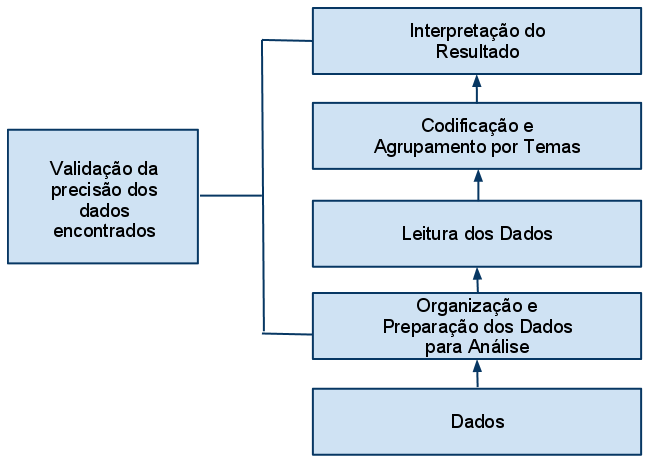
\includegraphics[scale=0.5]{analisedados}
  \caption{Processo de análise dos dados}
  \label{fig:analise-dados}
\end{figure}

 %% ------------------------------------------------------------------------- %%
\section{Validade e Confiabilidade do Estudo}
\label{sec:planejamento-validacao}

Para garantir a confiabilidade deste estudo, nós realizamos os
seguintes procedimentos:

\begin{itemize}
	\item \textbf{Checar as transcrições}. O objetivo é garantir que nenhum erro
	óbvio seja cometido;

	\item \textbf{Verificação de pesquisador auxiliar}. Um pesquisador auxiliar
	checará a interpretação dos dados gerada por esta pesquisa;
	
	\item \textbf{Rastreabilidade dos dados}. Todos os dados colhidos são
	preservados em forma eletrônica.

\end{itemize}

A validade do estudo será buscada por alguns procedimentos executados pelos
pesquisadores, dentre eles:

\begin{itemize}
	\item \textbf{Triangulação de diferentes fontes de dados}. A pesquisa foi
	realizada com participantes que possuem diferentes experiências, e diferentes
	fontes de dados serão colhidas, como questionários, entrevistas, código gerado e 
	opinião do especialista;

	\item \textbf{Prover descrição rica e detalhada sobre o ambiente}. A riqueza
	dos detalhes mostra a qualidade do estudo, além de possibilitar a repetição do
	experimento por outros pesquisadores;

	\item \textbf{Esclarecer todos os possíveis vieses da pesquisa}. A pesquisa
	deixa claro quais são suas limitações. Todas elas são discutidas no Capítulo
	\ref{cap:ameacas}.

\end{itemize}

Em resumo, o principal meio de validação do estudo foi o rico detalhamento dos
participantes, dos dados colhidos e instrumentos de coleta, de forma
que qualquer pesquisador interessado em replicar o experimento terá um
arcabouço sólido para comparação \cite{merriam-1998}. A análise de
dados também foi relatada em detalhes para que os leitores tenham uma visão
clara sobre o método utilizado na pesquisa. 
Além disso, essa pesquisa também é acompanhada pelo orientador do pesquisador,
que constantemente valida e discute os pontos levantados nesse planejamento.

%% ------------------------------------------------------------------------- %%
\section{Papel do Pesquisador}
\label{sec:planejamento-papel}

Em um estudo qualitativo, o pesquisador tem como papel fundamental participar do 
processo de captura dos dados, bem como seu preparo e interpretação final.
Creswell \cite{creswell}, citando Locke \cite{locke}, lembra
que a contribuição do investigador para o contexto da pesquisa pode ser útil e
positiva. Além do mais, o pesquisador é responsável por
identificar todos os valores pessoais, pressuposições e vieses deste estudo.

O autor desta pesquisa tem formação em Ciência da Computação, e desenvolve software há 9
anos, pratica TDD diariamente nos últimos 3 anos, e possui profundos
conhecimentos teóricos e práticos sobre orientação a objetos e métodos ágeis.
Além disso, o autor palestrou sobre TDD em eventos da indústria brasileira
de desenvolvimento de software, como a Agile Brazil 2010, o .NET Architects
2010 e o QCON São Paulo 2010. O autor desta pesquisa acredita que sua experiência nessas
áreas aumentam sua capacidade de análise dos efeitos de TDD no projeto de classes de sistemas 
orientados a objetos.

%% ------------------------------------------------------------------------- %%
\section{Problemas Éticos}
\label{sec:planejamento-etica}

Esta pesquisa pode revelar desenvolvedores que produzem projeto de classes não
satisfátorios ou não utilizam a prática corretamente.
Por esse motivo, todos os dados colhidos pelo pesquisador serão mantidos em
sigilo e todos os nomes de desenvolvedores e projetos omitidos, conforme acordo 
assinado entre o pesquisador e a participante.

%% ------------------------------------------------------------------------- %%
\section{Estudo piloto}
\label{sec:estudo-piloto}

Antes da execução do estudo com participantes reais, um estudo piloto foi
executado para que o pesquisador pudesse validar todos os instrumentos de pesquisa,
como exercícios, gravação de vídeo, protocolo e roteiro de entrevista.

Com os resultados do estudo piloto, o pesquisador fez melhorias
nos diversos instrumentos de pesquisa.
Vale ressaltar que as pessoas que participarem do estudo piloto não foram reutilizados no
estudo final.

Na primeira versão, o participante deveria implementar todos os quatro exercícios em 2 horas.
Mas, após a execução do primeiro piloto, o participante nos contou que se sentiu muito cansado, e
que, ao final, não estava mais trabalhando direito. Por esse motivo, decidimos que
os participantes resolveriam apenas 2 exercícios.

No segundo piloto, o participante teve dificuldades para configurar a área de trabalho no Eclipse e
para entender o que deveria fazer em cada exercício. Para resolver este problema, adotamos um 
caderno de questões bem explicado, além de sugerir ao participante o \textit{download} de uma
área de trabalho do Eclipse previamente configurada.
O mesmo participante também comentou que os exercícios poderiam ser simplificados. Essa sugestão
não foi aceita, já que queríamos que os exercícios fossem parecidos com os do mundo real. No entanto,
passamos a avisar aos participantes que eles não precisavam necessariamente terminar o exercício,
mas sim trabalhar com qualidade.

Já o terceiro piloto nos ajudou a melhorar o roteiro de entrevista. Percebemos a existência de diversas perguntas
repetidas. Após o término, removemos essas questões e deixamos o roteiro de entrevistas mais simples.

\section{Execução do estudo}
\label{subsec:particularidades-execucao}

Como os estudos foram executados fisicamente em muitas das empresas selecionadas,
nós acabamos por ajudar na organização do ambiente, mesmo a equipe tendo 
recebido o caderno de questões, com as instruções da instalação
alguns dias antes. A ideia era também gravar a implementação dos alunos,
mas dificuldades em se encontrar um software de vídeo para as diferentes
plataformas, e arquivos muito grandes, impossibilitaram a gravação.

Todos os participantes eram avisados de que tinham por volta de 50 minutos
por exercício. Eles também sabiam que, mesmo que não terminassem o exercício,
deveriam focam sempre na qualidade do código gerado. Eles também eram solicitados
a implementar um projeto de classes flexível para os problemas. A frase que dizíamos para
eles era geralmente: \textit{"Levem os exercícios para o mundo real, onde um outro
desenvolvedor deverá manter o código gerado. Lembrem-se de implementar o código mais fácil possível
para evoluir. As regras de negócio que existem hoje no enunciado tendem a aumentar
de número e, portanto, deixem a manutenção do código de vocês mais simples."}

Durante a execução, nós tirávamos diversas dúvidas sobre enunciados dos
exercícios, e até mesmo sobre procedimentos que os participantes podiam
adotar durante a execução. Um deles, por exemplo, perguntou se poderia
refatorar o código durante a implementação sem TDD. 
Nós também não os pressionávamos em nenhum momento. Eles ficavam,
cada um suas máquinas, trabalhando na implementação. Não ficávamos 
passando atrás das máquinas para ver como estavam indo, na tentativa
de evitar qualquer possível alteração de comportamento pela nossa presença.
Ao final de cada intervalo de 50 minutos, nós avisámos para eles finalizarem
a linha de raciocínio e partir para o próximo exercício.
Apesar de não haver nenhuma restrição explícita sobre isso, não houveram
conversas entre os participantes. Todos eles trabalharam sozinho
durante toda a implementação.

Todo o experimento ocorreu bem, com exceção do que foi executado
dentro da universidade. Além de diversos problemas de infra-estrutura,
como a falta de espaço disponível para alguns alunos, que impedia até mesmo
o JUnit de executar, todos os participantes conseguiram fazer apenas
1 exercício. Diante desta situação, optamos por deixá-los implementar
o mesmo exercício até o final da aula já que, após os 50 minutos iniciais,
nós observamos que pouco código havia sido escrito. Outro problema levantado
foi que alguns alunos não se mostraram muito dispostos a participar
do estudo.
Ao contrário, a grande maioria dos participantes da indústria conseguiram
implementar o exercício no tempo delimitado, e todos se mostraram
muito receptivos para o estudo. Um ponto que se mostrou bem útil
para convencer participantes da indústria a participar foi a proposta
posterior de nós apresentarmos os resultados encontrados em uma palestra.

Ao final da execução do estudo em cada empresa, nós colhetávamos
os dados gerados (código-fonte e caderno de questões assinado),
e dávamos o nome da pasta do participante, de acordo com
o seguinte formato: \textit{id-nome-combinação}. O id aponta
para um número único do participante no estudo, e a combinação
aponta quais exercícios ele resolveu, bem como em qual deles
ele utilizou TDD.

As entrevistas foram, em grande parte, realizadas pessoalmente com 
o desenvolvedor. Quando o participante não estava disponível (por estar
localizado em outra cidade), a entrevista era realizada por Skype.
Durante toda a entrevista, o participante podia observar o código que
produziu. Para isso, nós criamos uma simples aplicação web para facilitar
a exibição dos códigos-fonte. O objetivo do participante ver o código
era lembrar sobre suas decisões, e nos possibilitar perguntas específicas
sobre o projeto de classes gerado.

Em média, as entrevistas levavam 30 minutos. Quando o participante comentava
algo interessante, nós fugíamos do roteiro para permitir que ele falasse mais do assunto,
e anotávamos o ponto para que, ao final, fosse possível discutir novamente sobre o assunto.
O roteiro de entrevistas sofreu uma pequena mudança ao final da primeira entrevista,
já que percebemos que comunicar ao participante que o código que ele produziu
\textit{não apresenta um bom projeto de classes} não era uma tarefa fácil, e talvez, não ética. 
Optamos por perguntar sobre como aquele projeto de classes foi construído, mesmo que ele
não estivesse bem construído.

Para manter um padrão, nós sempre perguntávamos primeiro sobre o exercício que ele
fez com TDD, independente da ordem que ele implementou no dia da execução. Notamos
que muitos participantes discutiram sobre os exercícios e possíveis implementações com seus colegas.

Dos três especialistas convidados a avaliar os códigos produzidos, apenas um não
completou a tarefa. Sugerimos a todos eles, antes do início da avaliação, que avaliassem
não só a quantidade de código escrito, mas as decisões de projeto de classes tomadas por aquele
participante. Para que os especialistas avaliassem cada código gerado, nós implementamos
uma simples aplicação web, onde eles tinham acesso a qualquer momento, e podiam parar ou continuar
a avaliar na hora que preferissem.